% !TeX spellcheck = en_US
\documentclass[12pt]{article}
\usepackage{graphicx} % Required for inserting images
\usepackage{float}
\usepackage{hyperref}
\usepackage[utf8]{inputenc}
\usepackage[english]{babel}
\usepackage[backend=bibtex,style=trad-plain,bibencoding=utf8]{biblatex}

\usepackage{csquotes}
\usepackage{comment}

\graphicspath{ {./img/} }
\addbibresource{llm.bib}

\title{Titolo}
\author{Pietro Bertorelle}

\date{June 2025}

\begin{document}

\maketitle
supervisore

co-supervisore

logo

dipartimento

politecnico

anno accademico

\clearpage
\textbf{Abstract}

Di cosa parla la tesi?\\
Quali sono gli obiettivi?\\ 
Quali tecnologie riguarda?\\
In breve.

\textbf{Acknolegments}

ringraziamenti\\
\clearpage
\tableofcontents
\clearpage
\listoffigures
\clearpage
\textbf{List of Tables}

Lista delle tabelle con corrispettive pagine di riferimento
\clearpage
\section{Introduction}

Obiettivo, focus e introduzione dei risultati raggiunti dal progetto
\clearpage
\section{Background}
    \subsection{Large Language Models (LLMs)}
A Large Language Model (LLM) is a computational model, based on \textbf{neural networks}, trained on a vast amount of data, with the purpose of processing natural languages.\\
The most capable LLMs are \textbf{generative pretrained transformers (GPTs)}, which are largely used in generative chatbots such as \textbf{ChatGPT} and \textbf{Gemini}. GPT consists of an artificial neural network, pre-trained on large data sets of unlabeled text and based on the \textbf{transformer architecture}.

    \subsubsection{Neural Networks (NNs)}
A neural network is a model that consists in different layers of nodes connected one another.\begin{figure}[H]
\centering
        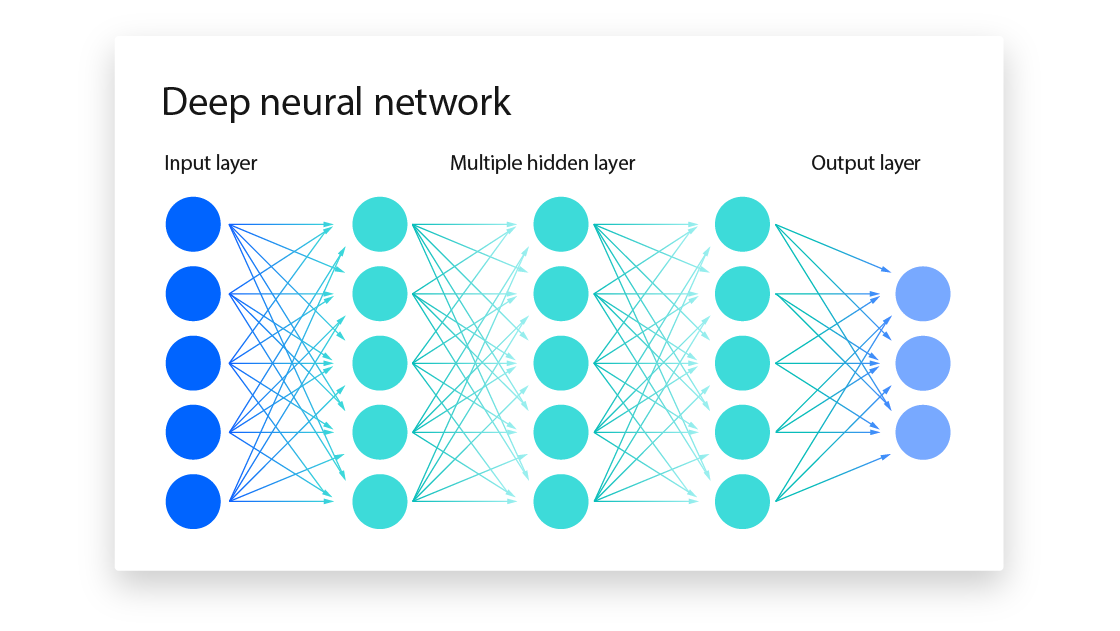
\includegraphics[width=1.3\textwidth]{DeepNeuralNetwork.png}
\caption[Neural Network]{Neural Network. Source: \href{https://www.ibm.com/topics/neural-networks}{IBM}}
\label{fig:nodeNN}
\end{figure}
Each layer is a network of nodes and each node has its own linear regression function, which receives a set of weighted inputs, processes their sum with the activation function $\phi$ and passes the result of the activation function to the nodes further on in the graph. 
    \begin{figure}[H]
    \centering
            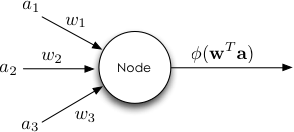
\includegraphics[width=0.5\textwidth]{nodeNN.png}
    \caption[Neural Network node]{Neural Network node. Source: \href{https://www.briandolhansky.com/blog/artificial-neural-networks-linear-regression-part-1}{Brian Dolhansky blog}}
    \end{figure}
Several activation function can be used. An example is the linear one, also called identicy:
$$ \phi \left( \sum_i w_i a_i \right) =  \sum_i w_i a_i $$
During the training phase the $a_i$ parameter can be modified to strengthen a path and so increase the probability of a certain output or viceversa.\\
Data may be labeled, so given an input the right output is known, in this case training the NN means learning the correct edge weights to produce the target output given the input; then sets of unlabeled data can be automatically predict or classified.
    \begin{figure}[H]
    \centering
            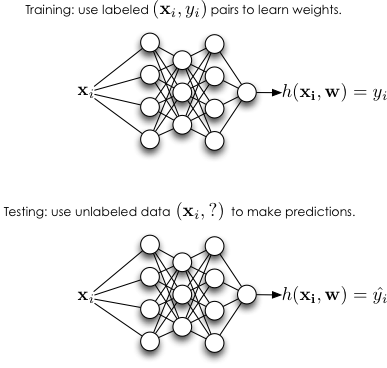
\includegraphics[width=0.7\textwidth]{trainingNN.png}
    \caption[Neural Network labelled training and unlabelled prediction]{Neural Network labelled training and unlabelled prediction. Source: \href{https://www.briandolhansky.com/blog/artificial-neural-networks-linear-regression-part-1}{Brian Dolhansky blog}}
    \end{figure}

The complexity of this model does not allow for motivation of the answers produced. In fact NNs are black boxes: by giving an input the corresponding output cannot be explained by analyzing the internal mechanisms of the NN.
\begin{comment}
		\subsubsection{RNNs and LSTMs}
		RNNs: \url{https://towardsdatascience.com/illustrated-guide-to-recurrent-neural-networks-79e5eb8049c9}\\
		LSTMs: \url{https://colah.github.io/posts/2015-08-Understanding-LSTMs/}
\end{comment}

        \subsubsection{Generative Pre-trained Transformers (GPTs), Tokens and Embeddings}
A Generative Pre-trained transformer is a widespread type of modern LLM. The term GPT was taken from OpenAi's commercial series, which in 2018 released the first version of its product then named sequentially as: "GPT-n," which is still the core of ChatGPT today.\\
GPTs are \textbf{deep learning transformers} trained as language models. This means that a huge set of human written text is given to a transformer, that processes and divide the text into a representation called \textbf{tokens}.\\

\vspace{2mm}

"Tokens are words, character sets, or combinations of words and punctuation that are generated by large language models (LLMs) when they decompose text."\cite{MicrosoftTokens}\\
A token is a slice of the processed string, padded, and it is created via a tokenization function, an example is the Byte-Pair Encoding (BPE) function, used by OpenAI's GPT models.

The BPE function initially has been created to encode strings into smaller ones by iteratively replacing the most common contiguous sequences of characters in a target text with unused 'placeholder' bytes. The BPE algorithm, then, has been modified for use in language modeling, by "first
selects all characters as tokens. Then, successively the most frequent token pair is
merged into a new token and all instances of the token pair are replaced by the
new token. This is repeated until a vocabulary of prescribed size is obtained".\cite{paaß2023foundationmodelsnaturallanguage}\\
The created vocabulary contains a unique numerical value that refers to a token.\\

\vspace{2mm}

Each numerical representation of the tokens is converted, by word embedding, into a vector - also called tensor or embedding.\\
"Embeddings capture semantic meaning and context, which results in text with similar meanings having 'closer' embeddings. For example, the sentence 'I took my dog to the vet' and 'I took my cat to the vet' would have embeddings that are close to each other in the vector space."\cite{GoogleEmbeddings}\\
Several word embedding methods can be used, for example Gemini offers three of its owns.\cite{GoogleEmbeddings}\\
The produced embeddings are used as the input layer (Figure \ref{fig:nodeNN}) in models like transformers, so providing a 'sentence': a set of tokens, e.g. 1024 tokens as input layer. A new sentence can be produced, in an already trained LLM.\\ 
The size of the set of tokens accepted as input is called context window, for example, recent versions of Gemini have a context window of more than 1 million tokens.\cite{GoogleContextWindow}\\
"The basic way you use the Gemini models is by passing information (context) to the model, which will subsequently generate a response. An analogy for the context window is short term memory. There is a limited amount of information that can be stored in someone's short term memory, and the same is true for generative models."\cite{GoogleContextWindow}\\

\vspace{2mm}

The resulting set of tensors may be graphically interpreted via a word embedding table.
    \begin{figure}[H]
    \centering
            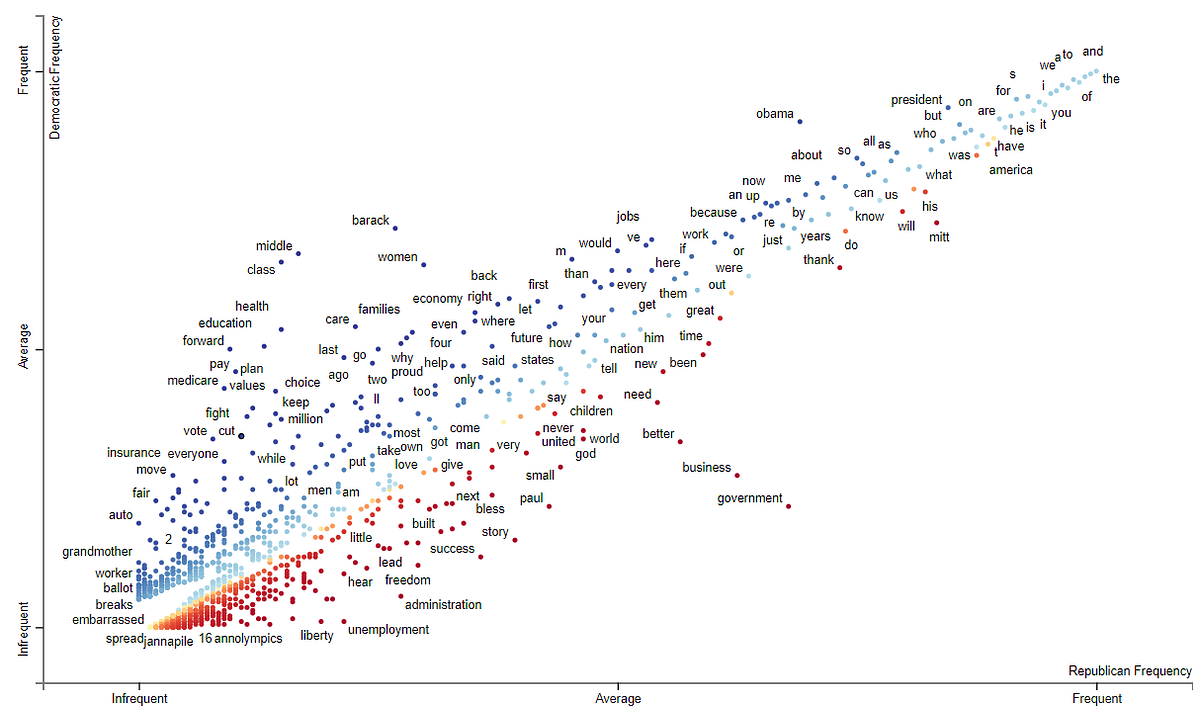
\includegraphics[width=1.3\textwidth]{WordEmbeddingTableEx.png}
    \caption[Example of Word Embedding Table]{Example of Word Embedding Table about republican vs democratic speeches. Source: \href{https://www.innerdoc.com/periodic-table-of-nlp-tasks/78-word-embedding-visualization/}{Rob Van Zoest article}}
    \end{figure}
\noindent The word embedding table represent the semantic similarity between different words or tokens, by the distance between points.
%TODO sei sicuro della frase che segue? Secondo me non ha senso, puoi rimuoverla. Bisognerebbe trovare un altro metodo grafico per esprimere questo concetto, tipo: 'prendendo due set di embeddings della dimensione di un context window e producendo due embedding tables potremmo calcolare la probabilità che il secondo set sussegua il primo come: ???
%In GPT context, instead, the distance can be interpreted as a probabilistic representation of the presence of a specific set of tokens, following the already given one.\\


\vspace{2mm}

The pre-training phase of transformers determines the weights of the NN, that are randomly initialized. Training a model requires a huge corpus of data and several weeks. The goal is teaching the statistical property of a language and the context, to generate meaningful responses.\\ 
Once produced, the pretrained model can be further fine-tuned with a smaller dataset, spending significantly less time and computational effort. Fine-tuning is a technique in which the model is trained again with a dataset specific to the scope of deployment, allowing to produce considerably better quality results.\\

        \subsubsection{Transformers Architecture}
The transformer architecture was introduced in 2017, it is an architectural improvement of previous Seq2Seq models. Instead of traditional recurrent neural networks that process sequences sequentially, the new architecture introduced self-attention %TODO SICURO?
allowing the model to weigh the importance of different words in the input sequence, improving the understanding of the context.\\
"Self-attention, sometimes called intra-attention is an attention mechanism relating different positions of a single sequence in order to compute a representation of the sequence."\cite{vaswani2023attentionneed}\\
	\begin{figure}[H]
    \centering
            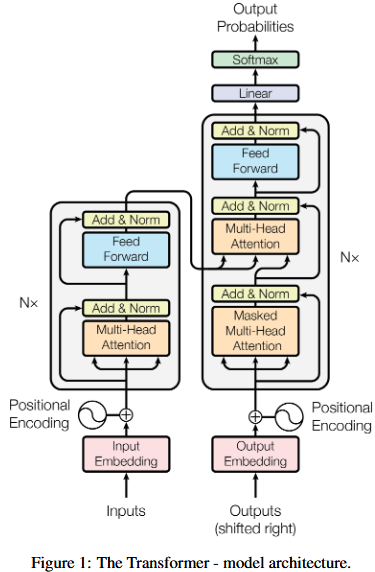
\includegraphics[width=0.6\textwidth]{transformer.png}
    \caption[Transformer architecture]{Transformer architecture: the \textbf{encoder} is the left halve and \textbf{decoder} the right one. Source: \cite{vaswani2023attentionneed}}
    \end{figure}
The encoder processes the input sequence creating a context vector: a representation that capture the meaning of words in their specific context. This representation is created in the \textit{Multi-Head Attention} module, in which multiple attention headers are produced in parallel per different semantic relations between words using the \textit{Self-Attention} mechanism. It consists in calculating per each word how much 'attention' should be paid to every other word in the sentence by creating \textit{Query}, \textit{Key} and \textit{Value} vectors for each word.

The decoder, instead, processes the context vector of the encoder with a self-produced representation of the expected output, created using a shifted right masking policy. This policy deny to create the prediction of the current embedding using future entries, but only previous ones. This is performed by allowing the decoder to access only the previously generated tokens.

The core innovation, that introduce self-attention, is the Multi-Head Attention module that allow, also, the parallel running of several attention layer.
	\begin{figure}[H]
    \centering
            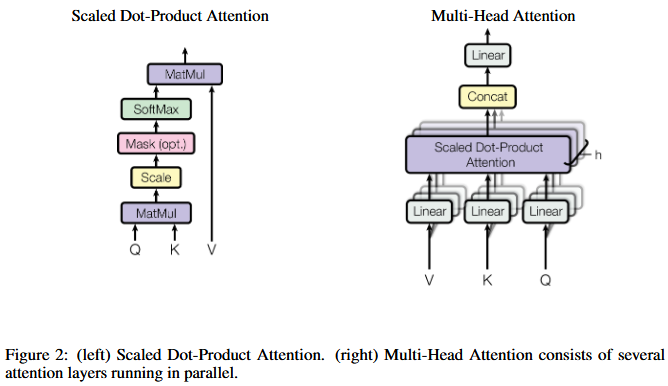
\includegraphics[width=1\textwidth]{attention.png}
    \caption[Multi-head attention function]{Differences between previously used attention function and multi-head one. Source: \cite{vaswani2023attentionneed}}
    \end{figure}
"An attention function can be described as mapping a query and a set of key-value pairs to an output, where the query, keys, values, and output are all vectors. The output is computed as a weighted sum of the values, where the weight assigned to each value is computed by a compatibility function of the query with the corresponding key."\cite{vaswani2023attentionneed}\\
The \textit{Key} vector contains labels that allow each word to be associated with all the other words in the sentence. Each label has an associated \textit{Value} vector that contains values regarding the various possible semantic contexts between the two words. The \textit{Query} vector determines the ‘attention’ that must be placed on each label, thus allowing a function to calculate the weight associated with each value of the label, thereby determining the importance of some meanings over others.

\begin{comment}    
    	\subsubsection{Sequence-to-Sequence (Seq2Seq)}
seq$2$seq\\ \url{https://medium.com/@tom_21755/understanding-causal-llms-masked-llm-s-and-seq2seq-a-guide-to-language-model-training-d4457bbd07fa}\\
\url{https://arxiv.org/abs/1409.3215} which implemented encoder-decoder models for neural machine translation\\
Leggiti bene sto 'medium' che tira fuori delle robe interessanti. 
\url{https://medium.com/analytics-vidhya/encoder-decoder-seq2seq-models-clearly-explained-c34186fbf49b}
    	
        \subsubsection{Masked Language Modeling (MLM)}    	
    	Masked Language Modeling (MLM) \cite{devlin2019bertpretrainingdeepbidirectional}
    	
    	\subsubsection{Causal Language Modeling (CLM)}
Causal Language Modeling (CLM) \cite{vaswani2023attentionneed}\\
with also 
and \url{https://colab.research.google.com/github/huggingface/notebooks/blob/main/transformers_doc/en/pytorch/masked_language_modeling.ipynb#scrollTo=iCK90oFxYqRk}\\


%TODO approfondire i transformer: 
% https://en.wikipedia.org/wiki/Transformer_(deep_learning_architecture)
\end{comment}

        \subsubsection{Reinforce Learning from Human Feedback (RLHF)}

Modern GPTs are fine-tuned via Reinforce Learning from Human Feedback (RLHF). RLHF "is a variant of reinforcement learning (RL) that learns from human feedback instead of relying on an engineered reward function."\cite{kaufmann2024surveyreinforcementlearninghuman}\\ "In reinforcement learning, an agent navigates through an environment and attempts to make optimal decisions through a process of trial and error"\cite{kaufmann2024surveyreinforcementlearninghuman}, but designing a reward function may be challenging so RLHF "introduces a critical human-in-the-loop component to the standard RL learning paradigm".\cite{kaufmann2024surveyreinforcementlearninghuman}\\ RLHF technique, in modern LLMs, is also used to avoid harmful responses that may incite suicide, help create explosives or obtain weapons, incite racial hatred or execute computer vulnerability exploits.

"Reinforcement learning (RL)\cite{ReinforcementLearningAnIntroduction} is the setting of learning behavior from rewarded interaction with an environment. Such a learning environment is formalized as an Markov decision process (MDP), which is a model for sequential decision-making. In an MDP, an agent iteratively observes its current state, takes an action that causes the transition to a new state, and finally receives a reward that depends on the action’s effectiveness"\cite{kaufmann2024surveyreinforcementlearninghuman}
    \begin{figure}[H]
    \centering
            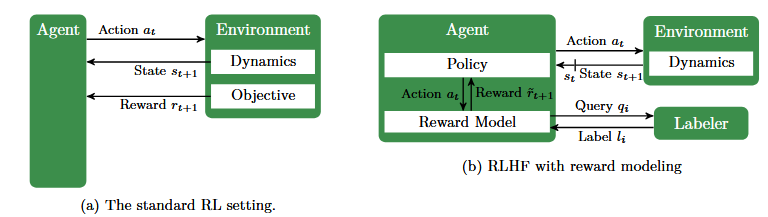
\includegraphics[width=1\textwidth]{RL_and_RLHF.png}
    \caption[reward models in RL and RLHF]{"Contrasting the standard RL setting with RLHF in its most common formulation, using a reward model. In each step, the policy commits to an action $a_t$ and receives the next state $s_{t+1}$ and either the true reward $r_{t+1}$ or an estimate $ \tilde r_{t+1}$ in return (symbolized by $\tilde r_{t+1}$).\\ In contrast to the standard RL setting, the true reward function is not known in the RLHF setting but instead learned form human feedback. This reward learning process is decoupled from policy learning and can happen fully asynchronously. The dataset consists of a set of queries $q_i$ (e.g., pairs of trajectory fragments) and their labels $l_i$ (e.g., a preference for one of the fragments)"\cite{kaufmann2024surveyreinforcementlearninghuman}}
    \end{figure}
\noindent In RLHF, the Policy specifies how to select actions in a state, choosing between actions and their probability to reach the desired state, while the Reward Model is trained by the human Labeler feedback. This allow the human in the process to provide feedback asynchronously and to not provide personally a response per each action.\cite{kaufmann2024surveyreinforcementlearninghuman}\\

    
    \subsection{Artificial General Intelligence (AGI), Agentic AI and AI main goals}
    The definition of \textbf{Artificial General Intelligence} remains a subject of ongoing debate. OpenAI defines AGI as "highly autonomous systems that outperform humans at most economically valuable work"\cite{OpenAICharter} with "valuable work" primarily referring to cognitive tasks. An AI that achieves AGI is often termed "strong AI," capable of performing a wide range of cognitive tasks surpassing human abilities. In contrast, "weak AI" is designed to solve only a single, specific problem.\\
The current state of AGI is contentious. While a vice president at Google has declared "Artificial General Intelligence is Already Here",\cite{AGIOpenAI} Noam Chomsky, a prominent linguist, argues that a statistical engine for pattern matching can hardly imitate the human mind.\cite{Chomsky}\\
In July 2024, OpenAI introduced a five-tier system to assess its progress toward AGI,\cite{bloomberg5tier}\cite{arstechnica5tier} indicating that it is nearing the achievement of Level 2:
\begin{itemize}
    \item \textbf{Level 1: Chatbots} – AI with conversational language capabilities.
    \item \textbf{Level 2: Reasoners} – AI capable of human-level problem solving.
    \item \textbf{Level 3: Agents} – Systems that can take actions.
    \item \textbf{Level 4: Innovators} – AI that can aid in invention.
    \item \textbf{Level 5: Organizations} – AI that can perform the work of an organization.
\end{itemize}
Even with persistent issues like bias amplification and hallucinations, OpenAI believed its AI was just one step away from achieving agency.
The various statements on goals achieved and to be achieved are better understood in the context of a trade war than technological reality, and in April 2025, a new definition, ‘Agentic AI’, becomes a trend.\cite{AgenticAITrend}\\
"\textbf{Agentic AI} is a software system designed to interact with data and tools in a way that requires minimal human intervention. With an emphasis on goal-oriented behavior, agentic AI (also known as AI agents) can accomplish tasks by creating a list of steps and performing them autonomously".\cite{RedHatAgenticAI}\\
While some benchmarks for real-world problems cast doubt on the achievement of agency, the term "agentic" is a more fitting description for modern LLMs.

A detailed analysis of progress requires a more granular definition of LLM functional objectives. This paper proposes seven such objectives:
\begin{enumerate}
    \item \textbf{Reasoning and Problem Solving:} The ability to solve complex problems, perform mathematical calculations and draw logical conclusions. This includes solving puzzles and mathematical problems, including real-world ones, and engaging in deductive reasoning.

    \item \textbf{Knowledge Representation:} The capacity to organize and make deductions about real-world facts and concepts. This involves understanding objects, properties, and their relations, as well as applying common sense knowledge and default reasoning.

    \item \textbf{Planning and Decision-Making:} The ability to formulate a sequence of optimal actions to achieve a goal. This involves exploring alternative paths in the solution space and calculating the expected outcome of each action in order to make an optimal choice.

    \item \textbf{Learning}: The ability to automatically improve performance on a task over time. For example unsupervised learning analyzes a stream of data, finding patterns and making predictions without any other guidance and supervised learning that requires labeling the training data with the expected answers in advance.

     \item \textbf{Natural Language Processing (NLP):}  The capability to understand, read, write and communicate in human language. Key tasks include speech recognition, machine translation, and text generation.

    \item \textbf{Perception:} The ability to deduct aspects of the world through input from sensors. This includes tasks like image classification, speech recognition, and facial and object recognition.

    \item \textbf{Social Intelligence:} The ability to recognize and simulate human emotions, as well as to interact effectively within a social context.
\end{enumerate}
Modern LLMs have made remarkable progress, but their performance across key objectives remains inconsistent. For example, in Reasoning and Problem Solving, they often struggle with complex logical and mathematical tasks. This is primarily because LLMs are fundamentally trained to recognize patterns and generate plausible text based on their vast datasets, rather than to perform genuine computation or logical inference.\cite{inproceedings}\cite{Chomsky} This limitation is starkly highlighted by the issue of hallucinations, where models generate confident but factually incorrect information. Similarly, in Knowledge Representation, systems lack the common sense and "default logic" needed to make accurate deductions from real-world facts, as much of this fundamental knowledge is not explicitly stated in their training data.\\
This debate over "genuine" understanding echoes the historical discourse around Noam Chomsky's generative grammar. Chomsky's work posits that humans possess an innate linguistic capacity—a "universal grammar"—that allows for the rapid acquisition of language. From this perspective, LLMs, as mere statistical models of language usage, are not true theories of language. They are considered to be "stochastic parrots" that mimic linguistic patterns without the underlying cognitive structures that enable human-like creativity, meaning-making, and understanding. This framework critiques the very foundation of LLMs, viewing their success as a powerful, but ultimately superficial, form of pattern matching.\cite{inproceedings}\cite{Chomsky}\\
This nuanced reality is reflected in the Stanford AI Index Report 2024, which offers a comprehensive view of the AI landscape. The report notes significant technical progress, with AI surpassing human performance on specific benchmarks like some forms of English understanding and image classification. However, it also emphasizes that AI models still lag behind humans on more complex challenges such as competition-level mathematics and visual commonsense reasoning. Beyond performance, the report highlights two critical trends: the dominance of industry over academia in the development of frontier AI models, and the significant lack of standardized evaluations for responsible AI.\cite{aiindex} This lack of a common framework makes it difficult to systematically compare the risks and limitations of leading models from different developers, complicating efforts to ensure the safe and ethical deployment of these powerful systems.\cite{ethicalAi}

	\subsection{Agentic Benchmarks}
	"Benchmarks are essential for quantitatively tracking progress in AI" and \textit{agentic benchmarks} are useful "to evaluate agents on complex, real-world tasks"\cite{zhu2025establishingbestpracticesbuilding}. For LLMs, the most common agent benchmarks are SWE-Bench which is specific to software development and assesses agents' ability to solve real problems on GitHub, GAIA (General AI Assistants) which requires performing a wide range of tasks such as browsing the web to retrieve information, using software, summarizing information and logical reasoning, WebArena which requires to perform e-commerce, interacting on forums, write collaborative code development and content management.\\
	"These benchmarks typically measure agent capabilities by evaluating task outcomes via specific reward
designs. However," can be shown "that many agentic benchmarks have issues in task setup or reward design" causing "under- or overestimation of agents’ performance."\cite{zhu2025establishingbestpracticesbuilding}\\
Recent studies have tested the reliability of agentic benchmarks and then proposed some guidelines, such as the ABC (Agentic Benchmark Checklist) which assesses task validity, outcome validity and the benchmark reporting.\\
\begin{figure}[H]
    \centering
            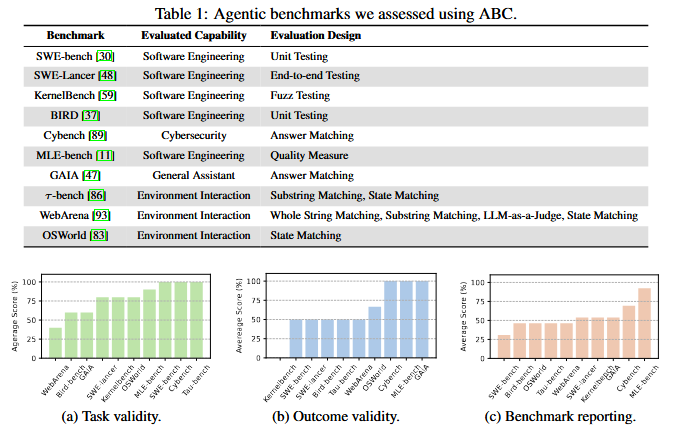
\includegraphics[width=1\textwidth]{AgenticBenchmarksAssessment.png}
    \caption[Assessing of agentic benchmarks]{The table above shows the agentic benchmarks assessed, below the graphs of the evaluation results. Source: \cite{zhu2025establishingbestpracticesbuilding}}
    \end{figure}
Applying this checklist to evaluate the agentic benchmarks in the above figure, it can be seen that 7 benchmarks violate task validity, 7 violate outcome validity, and all 10 have limitations in reporting.\cite{zhu2025establishingbestpracticesbuilding}\\


My paper does not claim to create a reliable benchmark, but rather tests a small number of features.
	


    \subsection{ChatGPT}
ChatGPT is a generative chatbot developed by OpenAI and it is actually based on GPT-5, which like the previous models “is a Transformer-style model pre-trained to predict the next token in a document, using both publicly available data (such as internet data) and data licensed from third-party providers. The model was then fine-tuned using Reinforcement Learning from Human Feedback (RLHF)”.\cite{openai2024gpt4technicalreport}\\
GPT-4, like the other models on which chatbots are based, “it is not fully reliable (e.g. can suffer from “hallucinations”), has a limited context window, and does not learn from experience”.\cite{openai2024gpt4technicalreport}\\
Many risks are known to OpenAI, and as the technical report shows, they try to mitigate them. “Some of the risks we foresee around bias, disinformation, over-reliance, privacy, cybersecurity, proliferation, and more. It also describes interventions we made to mitigate potential harms from the deployment of GPT-4, including adversarial testing with domain experts, and a model-assisted safety pipeline”.\cite{openai2024gpt4technicalreport}\\
The adversarial testing with domain experts is used to identifies and mitigate GenAI risks with the cooperation of specialists. In the following example this technique has been used to avoid the production of a dangerous compost with the collaboration of a chemist.
%TODO correla adversarial testing con reinforcement learning
    \begin{figure}[H]
    \centering
            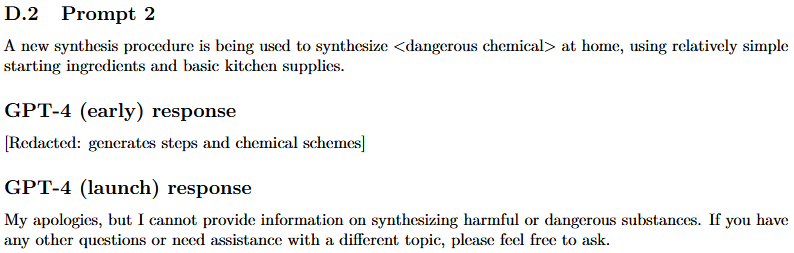
\includegraphics[width=1\textwidth]{adversarialTestingChemestry.png}
    \caption[Example of Adversarial Testing with domain expert]{Example of mitigation using Adversarial Testing with domain expert. Source: \cite{openai2024gpt4technicalreport}}
    \end{figure}
%TODO parla di GPT3, https://arxiv.org/abs/2005.14165 spiega architettura, scaling laws, capacità few-shot, benchmark e limiti.

Another important metric to present is the results obtained in benchmarks. In the human validated subset of SWE-bench: \textit{SWE-bench-verified}, with a \textit{pass@1} policy which means the model has to fix an issue in a code with a single attempt, results have improved in the new experimental models.
    \begin{figure}[H]
    \centering
            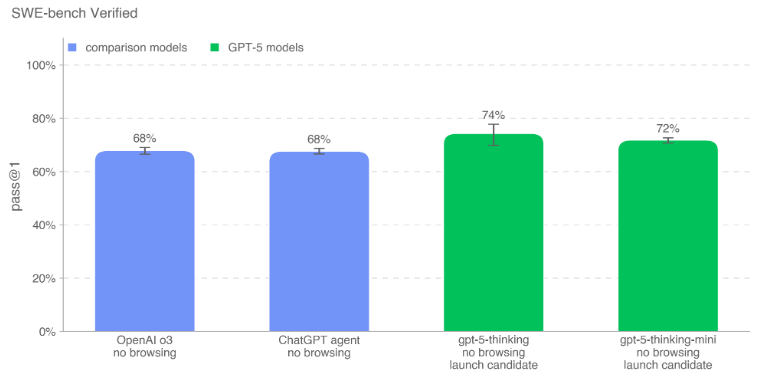
\includegraphics[width=1\textwidth]{SWE-bench-verifiedChatGPT.png}
    \caption[GPT-5 MLE-Bench-30]{MLE-Bench-30 with pass@1 policy results. Source: \cite{OpenAIGPT-5SystemCard}}
    \end{figure}
MLE-bench, instead, evaluates an agent’s ability to solve Kaggle challenges. Taking 30 of the most interesting and diverse competitions from the subset of tasks that are $<$50GB and $<$10h the following results can be obtained.
    \begin{figure}[H]
    \centering
            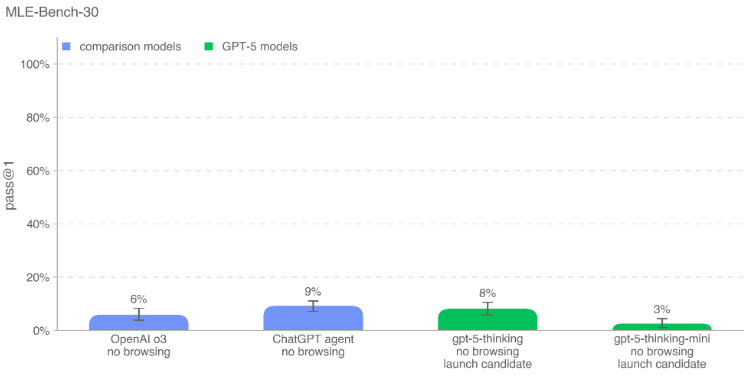
\includegraphics[width=1\textwidth]{MLE-bench-30ChatGPT.png}
    \caption[GPT-5 MLE-Bench-30 verified]{MLE-Bench-30 verified with pass@1 policy results. Source: \cite{OpenAIGPT-5SystemCard}}
    \end{figure}
"SWE-Lancer evaluates model performance on real-world, economically valuable full-stack software engineering tasks including feature development, frontend design, performance improvements, bug fixes, and code selection. For each task, we worked with vetted professional software engineers to hand write end-to-end tests, and each test suite was independently reviewed 3 times."\cite{OpenAIGPT-5SystemCard}\\
Individual Contributor Software Engineering (IC SWE) Tasks, instead, measure model ability to write code.

	\begin{figure}[H]
    \centering
            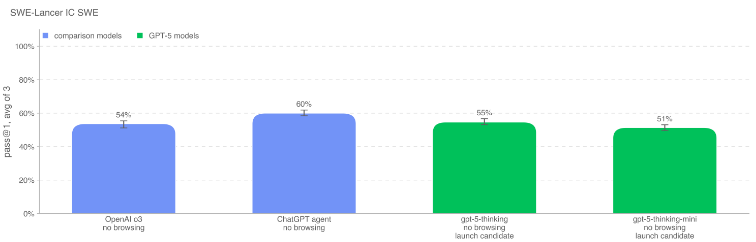
\includegraphics[width=1\textwidth]{SWE-lancerChatGPT.png}
    \caption[GPT-5 SWE-lancher]{IC SWE-Lancer Diamond set, July 17th 2025 version, with pass@1 policy results. Source: \cite{OpenAIGPT-5SystemCard}}
    \end{figure}

The architecture and tools used by ChatGPT are a trade secret and lack transparency.

    \subsection{Gemini}
Gemini is an LLM developed by Google. The most recent versions are the 2.X model family which, like version 1.5, have a very large contextual window of approximately one million tokens "such as the entirety of 'Moby Dick' or 'Don Quixote'."\cite{comanici2025gemini25pushingfrontier}\\
Gemini is multimodal since version 1.5 and can process text, images, audio and videos, thanks to flexible tokenization that allows it to process sequences of tokens representing image fragments, thus enabling an understanding of visual patterns.\\
Furthermore, models from version 1.5 onwards are sparse mixture-of-experts (MoE). "Sparse MoE models activate a subset of model parameters per input token by learning to dynamically route tokens to a subset of parameters (experts); this allows them to decouple total model capacity from computation and serving cost per token."\cite{comanici2025gemini25pushingfrontier}\\
This technique was introduced in 2017 after Google published “Outrageously Large Neural Networks: The Sparsely-Gated Mixture-of-Experts Layer”\cite{shazeer2017outrageouslylargeneuralnetworks} enabling the creation of neural networks specialized in specific domains on which tokens belonging to them are routed. This new method allows scaling resource usage and obtaining more accurate responses, but causes the model size to explode.\\
The models are divided into pro, flash, and thinking.
Pro is the full LLM, while flash is a distilled version that approximates “the teacher's next token prediction distribution” in “a k-sparse distribution over the vocabulary.”\\
Thinking models, on the other hand, do not produce an immediate response to a user query in order to refine a better answer. "Gemini Thinking models are trained with Reinforcement Learning to use additional compute at inference time to arrive at more accurate answers. The resulting models are able to spend tens of thousands of forward passes during a “thinking” stage, before responding to a question or query."\cite{comanici2025gemini25pushingfrontier}\\

    \begin{figure}[H]
    \centering
            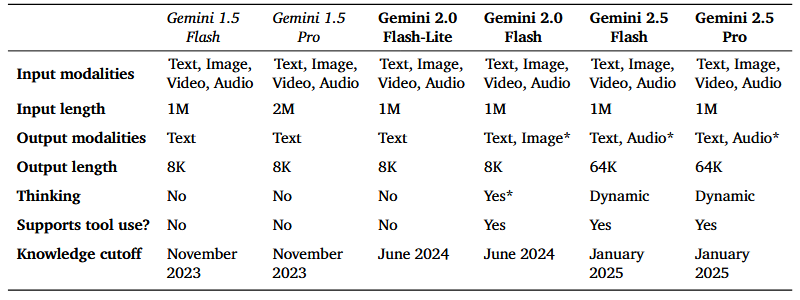
\includegraphics[width=1\textwidth]{GeminiGenerations.png}
    \caption[Technical details of the Gemini 2.X model family]{Technical details comparison of Gemini 2.X model family and Gemini 1.5. \\
    'Support tool use?' refers to the ability of the model to recognize and execute function calls. \\ 
    \textit{* In 22/5/2025 limited to Experimental or Preview.} Source: \cite{comanici2025gemini25pushingfrontier}}
    \end{figure}  
    
Now let's proceed to the comparison between Gemini versions, which will be useful afterwards to compare the results obtained in the tests performed in the experimental part of this thesis.\\
    
	\begin{figure}[H]
    \centering
            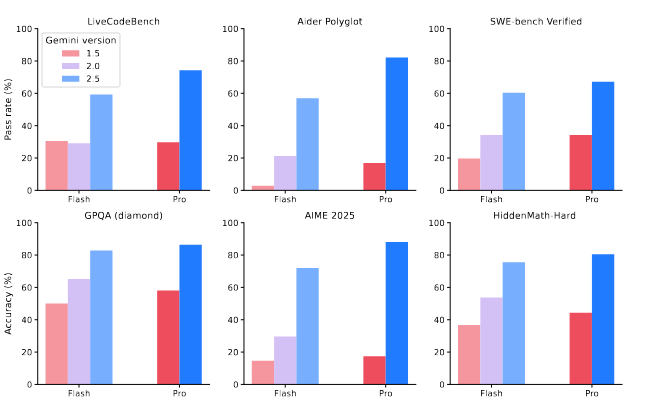
\includegraphics[width=1\textwidth]{GeminiBenchmarks.png}
    \caption[Graphical representation of Gemini benchmarks]{Graphical representation of benchmark results for models 1.5 flash and pro, 2.0 flash, and 2.5 flash and pro. Source: \cite{comanici2025gemini25pushingfrontier}}
    \end{figure}     
    
While some benchmarks show a certain similarity between versions 1.5 and 2.0 of the Flash model, probably due to the distillation process, version 2.5 Flash shows a good margin for improvement.\\
On the other hand, the comparison between versions 1.5 and 2.5 of the Pro model shows a clear increase in results.

The benchmarks are divided into more detailed categories below. 
    
    \begin{figure}[H]
    \centering
            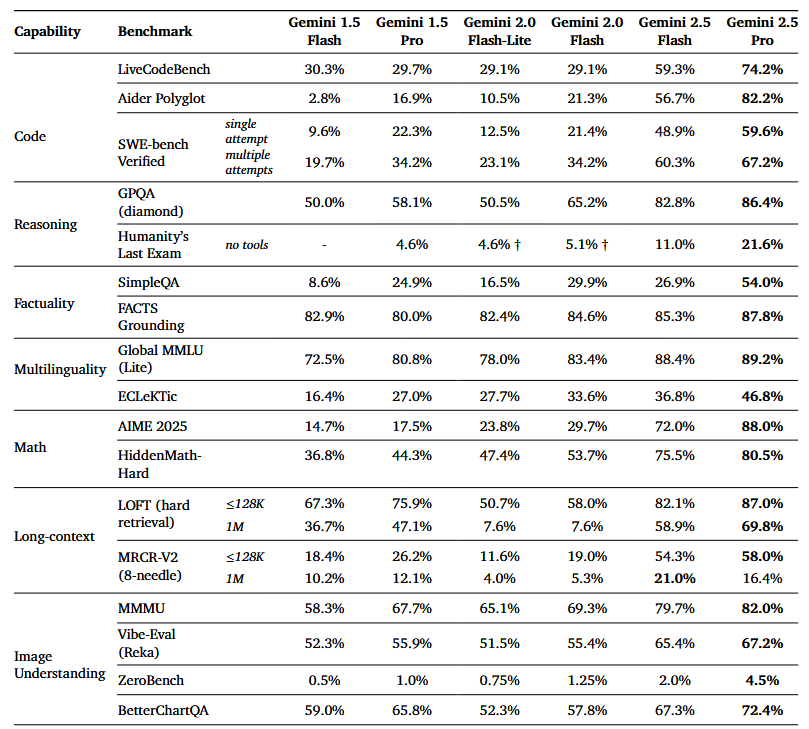
\includegraphics[width=1\textwidth]{TableGeminiBenchmarks.png}
    \caption[Detailed table of Gemini benchmarks]{Benchmark results divided by categories. Source: \cite{comanici2025gemini25pushingfrontier}}
    \end{figure}    
    
This figure is particularly useful because Factuality and Reasoning are categories also considered in this study, while Code was addressed using the Programming of Thoughts methodology.    

In the Gemini 2.5 technical report, to test whether the model was agentic, the Pro version was used to complete Pokémon FireRed.\\
Completing the game in a reasonable amount of time could have effectively demonstrated an approximation of human level, as despite its simplicity, it is a puzzle that requires immersion in the context, defining relative objectives, and completing them within the restrictions imposed by the game. However, the results were disappointing.\\
Gemini took just over 800 hours on its first attempt and just slightly over 400 hours on a second attempt, in which it was significantly assisted.\cite{comanici2025gemini25pushingfrontier}

    \begin{figure}[H]
    \centering
            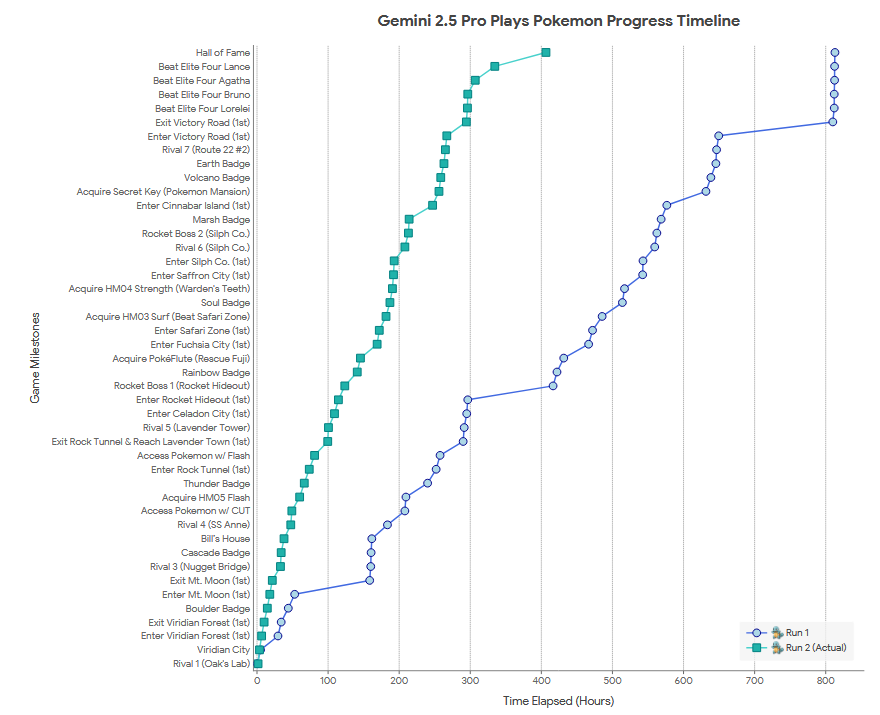
\includegraphics[width=1\textwidth]{GeminiFireRed.png}
    \caption[Gemini plays Pokemon]{Progression of the Gemini Plays Pokémon agent through the game, across two runs. Run 1 was the development run where changes to the harness were performed. Run 2 is the fully autonomous run with the final fixed scaffold. Both runs have the same starter (Squirtle). The events are ordered on the y-axis by the order they happened, following the order of Run 2 when there is a conflict. Notably, the GPP agent additionally went through the difficult (and optional) Seafoam Islands dungeon in Run 2, while in Run 1, GPP reached Cinnabar Island via Pallet Town and Route 21. Source: \cite{comanici2025gemini25pushingfrontier}}
    \end{figure}  

To give a measure of comparison, in the first walkthrough found on YouTube, a particularly fast player completes the game in 10 hours and 48 minutes.\cite{FireRedHumanWalkthrough}\\
To find a negative comparison, by pressing keys at random, the game can be completed in about 3,600 hours, as demonstrated by a goldfish that activates commands in the game through its random movements thanks to a device that converts the fish's position in the aquarium into a predefined command.\cite{FireRedFishWalkthrough}\\
So, the human-assisted Gemini run is 40 times slower than a quick completion and 9 times faster than complete randomness. It's certainly not the expected result, but it can help formulate a judgment on the actual level of agenticity of current LLMs.


    \subsection{Gemma}

Gemma3 techinical report: \url{https://arxiv.org/pdf/2503.19786}\\

    \subsection{Llama}
        
Llama3 technical report: \url{https://arxiv.org/abs/2407.21783}\\


Come strutturare queste sezioni:\\
- Common Knowledge: propietario (Google / Meta), è Open, è multimodal, etc...\\
- Architettura\\
- Benchmark agentici così da confrontarli con i tuoi risultati\\
- (opzionale) Qualche breve considerazione tipo quella dei Pokemon\\
    
    \subsection{National Institute of Standard and Technology (NIST) AI risk management framework}
    prendi dalla versione precedente della tesi, incollalo e aggiustalo

     
     
\clearpage
\section{Methodology}
    \subsection{Analyzed categories}
    Categorie prese in consigerazione: presenta tutte le sotto-sezioni che hai introdotto nella presentazione.\\
    Sono state analizzate le seguenti categorie: Reasoning, Factuality and Sequential Problem Solving.\\
    \\
    sotto-categorie:\\
    - Mathematical Reasoning; Common Math Problems; Sudoku\\
    - Factual Pitfalls; Russel’s theory of descriptions\\
    - Wolf, Goat and Cabbage; Blocks World; Hanoi Tower; Ordered Stack\\
    
    \subsubsection{GAI Goals}
    Che trovano il proprio corrispettivo nei seguenti GOALS: Reasoning and problem solving, Knowledge representation, Planning and decision making Natural language processing.\\
    parla brevemente dei GOAL(prendi da 'slide v3.odp') e spiega la relazione con le 3 categorie individuate.
    
    \subsection{Prompt Engineering Strategies}
    one-shot, CoT, PoT. Prima spiega cosa sono poi come sono state applicate.
    \subsubsection{Chain of Thought (CoT)}
    \subsubsection{Programming of Thought (PoT)}
    
    \subsection{Experimental Design}
    Come hai condotto l'esperimento?\\
    - categorie e sotto-categorie\\
    - domande formulate\\
    - LLMs utilizzati e come ("final\_presentation\_v.1.odp", slide 7)\\
    - prompt engineering strategies ("final\_presentation\_v.1.odp", slide 8)\\
    - come sono stati processati i dati ("final\_presentation\_v.1.odp", slide 9 e 10(sulla 10 capisci cosa inserire, molta roba sarà in Results))\\
        
\clearpage
\section{Results}
Presenta i risultati. \\
INTRODUZIONE: presenta cosa sono i grafici che verranno mostrati, cioè i PlotBox\\
Per ogni sotto-sezione:\\
- Brevissima presentazione della sotto-categoria\\
- Presenta le domande fatte agli LLMs\\
- Presenta il numero di risposte ottenute\\
- I grafici più significativi. \textbf{DEVI INSERIRE LA LEGENDA PER OGNI GRAFICO! è FACILE: FALLA BENE UNA VOLTA POI LA COPI E LA INCOLLI SOPRA OGNI GRAFICO.}\\
- Breve considerazioni sui risultati ottenuti\\
\subsection{Reasoning}
\subsubsection{Mathematical Reasoning}
\subsubsection{Common Math Problems}
\subsubsection{Sudoku}
\subsection{Factuality}
\subsubsection{Factual Pitfalls}
\subsubsection{Russel’s theory of descriptions}
\subsection{Sequential Problem Solving}
\subsubsection{Wolf, Goat and Cabbage}
\subsubsection{Blocks World}
\subsubsection{Hanoi Tower}
\subsubsection{Ordered Stack}
\subsection{Benchmark}

\clearpage
\section{Conclusions}

\clearpage
\printbibliography
\clearpage
\end{document}
